\chapter{XML}
\section{Beschreibung}
XML, kurz für {\em Extensible Markup Language}, ist eine
Auszeichnungssprache zur Darstellung und zum Austausch von
\enquote{hierarchisch strukturierten Daten}\cite{wiki:de:xml}. Das
{\em Extensible Language} rührt daher, dass der Entwickler selber
definieren kann beziehungsweise muss, welche {\em Mark-up Elemente} in
dem jeweiligen Dokument erlaubt sind. XML stellt somit nur eine
Metasprache für das festlegen einer eigenen Sprache dar. Wie dieses
Festlegen geschieht, wird im späteren Verlauf dargestellt.

\section{Aufbau}
\lstset{language=XML,
  numbers=left,
  stringstyle=\ttfamily,
  frame=box,
  rulesepcolor=\color{grey},
  basicstyle=\small
}
\lstset{caption=XML-Dokument; Quelle: http://de.wikipedia.org/wiki/XML\cite{wiki:de:xml}}
\lstinputlisting{code/examples/xml.xml}

\section{Schemasprachen}
Schemasprachen dienen dazu, die Struktur von XML-Sprachen zu
beschreiben und somit anzugeben, welche Elemente wo und wie vorkommen
dürfen. Wir werden hierbei auf die zwei bekanntesten, DTD und XML-Schema, eingehen.
(\enquote{Die zwei bekanntesten sind DTD und XML Schema.}\cite{wiki:de:xml})
\subsection{DTD}
DTD, kurz für Dokumenttypdefinition, wurde zur selben Zeit wie XML
standardisiert, und somit zu einer Zeit, in der XML-Dokumente noch
größtenteils "`erzählend"' waren und nicht zum Datenaustausch dienten.
Daher ist es z.\,B. nicht möglich, zwischen Texten und Zahlen zu
unterscheiden.

\subsection{XML-Schema}
XML-Schema, oder auch XSD für XML-Schema-Definition, ist die heutige
Möglichkeit, eine XML-Sprache zu beschreiben. Sie erlaubt es,
\enquote{den Inhalt von Elementen und Attributen zu
  beschränken}\cite{wiki:de:xml}, sprich zwischen Texten, Zahlen,
Daten und ähnlichem zu unterscheiden und ist zu dem selber ein
XML-Dokument und erlaubt somit auch komplexere Beschreibungen.

\section{XPath}\label{xpath}
XPath ist eine der zahlreichen Möglichkeiten, gezielt durch ein XML
Dokument zu navigieren und ist somit für uns im Groben mit SQL zu
vergleichen. Da es in XML weder Tabellen noch Spalten oder Zeilen
gibt, ist die Art und Weise, wie einzelne Elemente ausgewählt werden,
natürlich grundverschieden von SQL.

So besteht ein XPath Ausdruck aus {\em Lokalisierungsschritten} und
{\em Prädikaten}, wobei Lokalisierungsschritte dazu dienen, durch den
Baum zu navigierend und dabei mindestens eins, unter Umständen eine
Menge von Elementen zu selektieren. Mittels Prädikaten wird die
Auswahl weiter eingegrenzt, in dem zum Beispiel die Textnodes, sprich
die "`Werte"' der Elemente, überprüft werden.

So wäre ein simples Beispiel die Auswahl aller Produkte, die 10 Euro
oder mehr kosten. Gegeben sei folgendes Dokument:

\lstset{
  language=XML,
  numbers=left,
  stringstyle=\ttfamily,
  frame=box,
  rulesepcolor=\color{grey},
  basicstyle=\small,
  caption=
}

\lstinputlisting{code/examples/xpath.xml}

\lstset{language=XSLT}

So würde folgender XPath Ausdruck alle Produkte mit dem Preis von 10
Euro (in unserem Fall genau ein Produkt) liefern:
\lstinline{//product[price = 10]} -- Hierbei bedeutet
\lstinline{//product} soviel wie "`alle Unterelemente mit dem Namen
product"' und \lstinline{price = 10} überprüft, ob in den gefundene
Elementen ein {\em price} mit dem Wert {\em 10} vorhanden ist.

{\small
  \begin{table}[hb]
    \caption{Achsen in XPath\cite{wiki:de:xpath}}
    \begin{tabularx}{\textwidth}{l|X|l}
      Achse & adressierte Knoten & Abkürzung \\
      \hline
      child & direkt untergeordnete Knoten & weglassen \\
      parent & der direkt Übergeordnete Elternknoten  & .. \\
      self & der Kontextknoten selbst (nützlich für zusätzliche Bedingungen) & . \\
      ancestor & Übergeordnete Knoten & \\
      ancestor-or-self & Übergeordnete Knoten inklusive des Kontextknotens & \\
      descendant & untergeordnete Knoten & \\
      descendant-or-self & untergeordnete Knoten inklusive des Kontextknotens & // \\
      following & nachfolgend im XML-Dokument (ohne untergeordnete Knoten) & \\
      following-sibling & wie following, und vom gleichen parent stammend & \\
      preceding vorhergehend & im XML-Dokument ohne Übergeordnete Knoten & \\
      preceding-sibling & wie preceding, und vom gleichen parent stammend & \\
      attribute & Attributknoten & @ \\
      namespace & Namensraumknoten, die aus dem Attribut xmlns stammen &
    \end{tabularx}
  \end{table}
}

\section{PHP}\label{xml-php}
Für uns von besonderem Interesse ist es natürlich, wie wir auf
einfache Art und Weise per PHP auf unsere XML Dateien zugreifen und
diese verwenden können. Hierfür gibt es seit PHP 5 einige
überarbeitete APIs\footnote{application programming interface} (vgl.
\enquote{PHP5 includes totally rewritten and new extensions, including
  the SAX parser, the DOM, SimpleXML, XMLReader, XMLWriter, and the
  XSLT processor. All these extensions are now based on the
  libxml2.}\cite{www:ibm:xml}), wovon vor allem zwei beliebt sind
(\enquote{Of the many APIs available in PHP5, the DOM and SimpleXML
  are the most familiar,}\cite{www:ibm:xml}). Und auf genau diese
beiden, DOM und SimpleXML werde ich im Näheren eingehen.
\subsection{DOM}
Das {\em Document Object Model}, kurz DOM, ist ein W3C\footnote{World
  Wibe Web Consortium} Standard für das Verarbeiten und Manipulieren
von HTML und XML-Dokumenten. Dabei wird das jeweilige Dokument als
(Stamm)Baum dargestellt und behält somit den logische Aufbau des
Ausgangsdokumentes bei. Hierbei ist zu beachten, dass DOM ein
sogenannter {\em tree-based} Parser ist und somit einen Baum vom
ganzen Dokument erstellt. Daher ist es eher ungeeignet, um große
Dokumente zu verarbeiten, da dies sonst viel Systemspeicher
beanspruchen würde (\enquote{Because DOM builds a tree of the entire
  document, it uses a lot of memory and processor time. Therefore,
  performance issues make it impractical to parse large documents with
  DOM.}\cite{www:ibm:xml}). Nichts desto trotz ist es generell die
bevorzugte Methode, um SGML/XML-Dokumente zu verarbeiten, wenn das
Hauptaugenmerk auf einem einfachen Interface liegt.
\begin{figure}[hb]
  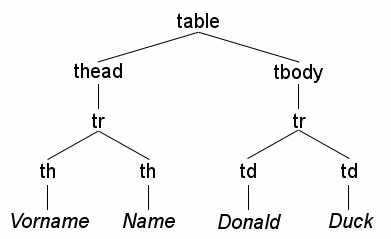
\includegraphics[width=0.5\textwidth]{images/dom}
  \caption{Der Baum einer einfachen (X)HTML Tabelle\cite{wiki:de:dom}}
\end{figure}

\subsection{SimpleXML}
SimpleXML ist eine Erweiterung, die mit PHP 5 eingeführt wurde und
unter PHP Programmierern als die einfachste Möglichkeit gilt, mit
kleinen und simpleren XML-Dokumenten zu arbeiten. Hierbei liest
SimpleXML das Dokument ein und stellt dem Entwickler ein Objekt zur
Verfügung, welches Zugriff auf die einzelnen Elemente erlaubt.
Erwähnenswert ist hierbei, dass SimpleXML in der Lage ist, mittels DOM
die Dokumente auch zu manipulieren und dank XPath eine einfache
Methode liefert, um durch das Dokument zu navigieren (vgl. Abschnitt
\ref{xpath}, Seite \pageref{xpath}).
